\documentclass[UTF8,a4paper,10pt]{ctexart}
\usepackage[left=2.00cm, right=2.00cm, top=3.50cm, bottom=3.50cm]{geometry} %页边距
\CTEXsetup[format={\Large\bfseries}]{section} %设置章标题居左
 
 
%%%%%%%%%%%%%%%%%%%%%%%
% -- text font --
% compile using Xelatex
%%%%%%%%%%%%%%%%%%%%%%%
% -- 中文字体 --
%\setmainfont{Microsoft YaHei}  % 微软雅黑
%\setmainfont{YouYuan}  % 幼圆    
%\setmainfont{NSimSun}  % 新宋体
%\setmainfont{KaiTi}    % 楷体
%\setmainfont{SimSun}   % 宋体
%\setmainfont{SimHei}   % 黑体
% -- 英文字体 --
%\usepackage{times}
%\usepackage{mathpazo}
%\usepackage{fourier}
%\usepackage{charter}
\usepackage{helvet}
\usepackage{amsmath, amsfonts, amssymb} % math equations, symbols
\usepackage[english]{babel}
\usepackage{color}      % color content
\usepackage{graphicx}   % import figures
\usepackage{subfig}
\usepackage{url}        % hyperlinks
\usepackage{bm}         % bold type for equations
\usepackage{multirow}
\usepackage{longtable}
\usepackage{booktabs}
\usepackage{epstopdf}
\usepackage{epsfig}
\usepackage{algorithm}
\usepackage{algorithmic} 
\usepackage{listings} 
\usepackage{xcolor}
\lstset{
    language=matlab,  %代码语言使用的是matlab
    frame=shadowbox, %把代码用带有阴影的框圈起来
    rulesepcolor=\color{red!20!green!20!blue!20},%代码块边框为淡青色
    keywordstyle=\color{blue!90}\bfseries, %代码关键字的颜色为蓝色,粗体
    commentstyle=\color{red!10!green!70}\textit,    % 设置代码注释的颜色
    showstringspaces=false,%不显示代码字符串中间的空格标记
    numbers=left, % 显示行号
    numberstyle=\tiny,    % 行号字体
    stringstyle=\ttfamily, % 代码字符串的特殊格式
    breaklines=true, %对过长的代码自动换行
    extendedchars=false,  %解决代码跨页时,章节标题,页眉等汉字不显示的问题
%   escapebegin=\begin{CJK*},escapeend=\end{CJK*},      
% 代码中出现中文必须加上,否则报错
    texcl=true}
\renewcommand{\algorithmicrequire}{ \textbf{Input:}}     % use Input in the format of Algorithm  
\renewcommand{\algorithmicensure}{ \textbf{Initialize:}} % use Initialize in the format of Algorithm  
\renewcommand{\algorithmicreturn}{ \textbf{Output:}}     % use Output in the format of Algorithm   

% -------------------------允许算法跨页-------------
\makeatletter
\newenvironment{breakablealgorithm}
    {% \begin{breakablealgorithm}
    \begin{center}
        \refstepcounter{algorithm}% New algorithm
        \hrule height.8pt depth0pt \kern2pt% \@fs@pre for \@fs@ruled
        \renewcommand{\caption}[2][\relax]{% Make a new \caption
            {\raggedright\textbf{\ALG@name~\thealgorithm} ##2\par}%
                \ifx\relax##1\relax % #1 is \relax
                    \addcontentsline{loa}{algorithm}{\protect\numberline{\thealgorithm}##2}%
                \else % #1 is not \relax
                    \addcontentsline{loa}{algorithm}{\protect\numberline{\thealgorithm}##1}%
                \fi
            \kern2pt\hrule\kern2pt
        }
  }{% \end{breakablealgorithm}
            \kern2pt\hrule\relax% \@fs@post for \@fs@ruled
        \end{center}
  }
\makeatother
 
\usepackage{fancyhdr} %设置页眉、页脚
%\pagestyle{fancy}
\lhead{}
\chead{}
%\rhead{\includegraphics[width=1.2cm]{fig/ZJU_BLUE.eps}}
\lfoot{}
\cfoot{}
\rfoot{}
%\pagestyle{empty} %删除所有页码
 
%%%%%%%%%%%%%%%%%%%%%%%
%  设置水印
%%%%%%%%%%%%%%%%%%%%%%%
%\usepackage{draftwatermark}         % 所有页加水印
%\usepackage[firstpage]{draftwatermark} % 只有第一页加水印
% \SetWatermarkText{Water-Mark}           % 设置水印内容
% \SetWatermarkText{\includegraphics{fig/ZJDX-WaterMark.eps}}         % 设置水印logo
% \SetWatermarkLightness{0.9}             % 设置水印透明度 0-1
% \SetWatermarkScale{1}                   % 设置水印大小 0-1    
 
\usepackage{hyperref} %bookmarks
\hypersetup{colorlinks, bookmarks, unicode} %unicode
 

\title{\textbf{数值代数第5章上机实验报告}}
\author{ 211840196 张博阳 }
\date{}


\begin{document}
    \maketitle
 
    \section*{摘要}
        \par
        本实验报告基于第5章所学求解非线性方程的数值理论知识,对上机实验题给出了相应的程序实现与执行情况,主要关注Newton法的收敛过程和收敛阶观察,并进行了切线法和割线法的数值表现比较。

    \section{前言}
        \par
        由于求解非线性方程在理论上仍没有对分布和根的重数清楚的刻画,数值方法求解变为实际问题的主要求解手段,但根的分布和重数又影响到数值方法的收敛性和收敛速度,相应求解办法相较线性情形都对算法和算力提出了更高的要求。本次数值实验对非线性方程的数值求解方法进行了代码实现,并作出了对应收敛过程的误差曲线,同时观察数值方法的收敛阶。
        
    \section{数学原理和程序设计流程}
        \par
        Newton方法是最常用的求解非线性方程的数值方法,选定迭代起点$x_0$,其迭代序列$\{x_k\}$是由
        $$
        g(x)=x-\dfrac{f(x)}{f'(x)}
        $$
        作出的Picard不动点序列。理论分析表明,若$f(x)$充分光滑,$x_*$是方程$f(x)=0$的根,Newton方法的收敛速度与$x_*$的重数有密切关系:
        \par
        1.若$x_*$为单根,那么Newton法局部至少平方收敛。
        \par
        2.若$x_*$为$m(m>1)$重根,那么Newton法仅局部线性收敛,渐进收敛速度为$1-\dfrac{1}{m}$。
        \par
        当$x_*$为$f(x)$的重根时,对Newon方法进行修正亦可获得高阶局部收敛:
        \par
        1.若重数$m$已知,Newton迭代公式可修改为
        $$
        x_{k+1}=x_k-m\dfrac{f(x_k)}{f'(x_k)}
        $$
        \par
        2.若重数$m$未知,可将方程$f(x)=0$等价为$F(x)=\dfrac{f(x)}{f'(x)}=0$滤去重根后进行Newton迭代,或直接执行Steffensen加速。
        \par
        根据Newton迭代公式
        $$
        x_{k+1}=x_k-\dfrac{f(x_k)}{f'(x_k)}
        $$
        其几何意义是在$\left(x_k,f(x_k)\right)$处作$f(x)$图像的切线
        $$
        y=f'(x_k)(x-x_k)+f(x_k)
        $$
        其与$x$轴的交点$x=x_k-\dfrac{f(x_k)}{f'(x_k)}$作为下一迭代点$x_{k+1}$,因此Newton法亦称为切线法。
        \par
        实际应用中导函数形式往往未知或计算难度较大,可用一阶差商$f[x_{k-1},x_k]$近似替代导数值$f'(x_k)$的计算,即
        $$
        x_{k+1}=x_k-\dfrac{f(x_k)}{f\left[x_{k-1},x_k\right]}=x_k-\dfrac{f(x_k)\left(x_k-x_{k-1}\right)}{f(x_k)-f(x_{k-1})}
        $$
        其几何意义是过$\left(x_{k-1},f(x_{k-1})\right)$和$\left(x_k,f(x_k)\right)$的$f(x)$图线割线与$x$轴的交点作为下一迭代点$x_{k+1}$,因此上述迭代法称为割线法。割线法对单根的收敛速度略慢于切线法,收敛阶为$\dfrac{1+\sqrt{5}}{2}$。
        
\section{实验结果和数据讨论}
    \subsection{练习6.5.1}
        \par
        练习6.5.1的实验结果如Figure 1,2所示,其中取$x_0=3$,真解$x_*=2$。据参考文献[1]习题2第36题结论并代值尝试,以$x_0=3$为初值的Newton迭代序列将单调下降到$f(x)=x^3-x^2-8x+12$的最大实根,为$x=2$。

        \begin{figure*}[htbp]
            \centering
            \includegraphics[width=14cm,height=10cm]{1_error.eps}
            \caption{误差曲线}
        \end{figure*}
        \begin{figure*}[htbp]
            \centering
            \includegraphics[width=14cm,height=10cm]{1_order.eps}
            \caption{取$p=1$对数值收敛阶的观察} 
        \end{figure*}

        \par
        \ 
        \par
        \ 
        \par
        \ 
        \par
        \ 
        \par
        \ 
        \par

        据图可见,真实误差对数随迭代步数呈线性速度下降,$\dfrac{e_{k+1}}{e_k}$随迭代的进行稳定在0.5左右,亦即Newton法的收敛阶为1,为线性收敛。
        \par
        直接计算
        $$
        f'(x)=3x^2-2x-8,f'(2)=0
        $$
        $$
        f''(x)=6x-2,f''(2)\neq 0
        $$
        从而$x=2$是$f(x)=0$的2重根,Newton法局部线性收敛,渐进收敛速度为$1-\dfrac{1}{2}=0.5$,这与数值实验结果是吻合的。

    \subsection{练习6.5.2}
        \par
        练习6.5.2的实验结果如Figure 3-5所示,其中$f(x)=\sin x+\dfrac{x^3}{6}-x$,取$x_0=0.3525$,真解$x_*=0$。
        \par
        采用未修正的Newton迭代
        $$
        x_{k+1}=x_k-\dfrac{f(x_k)}{f'(x_k)}
        $$
        求解方程$f(x)=0$的实验结果如Figure 3,4所示。经多次尝试,由于舍入误差的影响,$\left|x_0\right|>0.35251$时迭代序列始终无法落入$\{x:\left|x\right|<\epsilon=10^{-6}\}$范围内,而$\left|x_0\right|\le 0.3525$时误差最终在舍入误差的影响下快速下降,结果最终计算为机器零。

        \begin{figure*}[htbp]
            \centering
            \includegraphics[width=14cm,height=10cm]{2_error_origin.eps}
            \caption{误差曲线}
        \end{figure*}
        \begin{figure*}[htbp]
            \centering
            \includegraphics[width=14cm,height=10cm]{2_order_origin.eps}
            \caption{取$p=1$对数值收敛阶的观察} 
        \end{figure*}
        据图可见,在舍入误差不明显的迭代过程中,真实误差对数随迭代步数呈线性速度下降,$\dfrac{e_{k+1}}{e_k}$稳定在0.8左右,亦即Newton法的收敛阶为1,为线性收敛。
        \par
        直接计算
        $$
        f^{(1)}(x)=\cos x+\dfrac{x^2}{2}-1,f^{(1)}(0)=0
        $$
        $$
        f^{(2)}(x)=-\sin x+x,f^{(2)}(0)=0
        $$
        $$
        f^{(3)}(x)=-\cos x+1,f^{(3)}(0)=0
        $$
        $$
        f^{(4)}(x)=\sin x,f^{(4)}(0)=0
        $$
        $$
        f^{(5)}(x)=\cos x,f^{(5)}(0)\neq 0
        $$
        即$x=0$是5重根,Newton法局部线性收敛,渐进收敛速度为$1-\dfrac{1}{5}=0.8$,与数值实验结果吻合。采用修正的Newton迭代
        $$
        x_{k+1}=x_k-5\dfrac{f(x_k)}{f'(x_k)}
        $$
        求解方程$f(x)=0$的实验结果如Figure 5所示,其中取$x_0=1$。
        \begin{figure*}[htbp]
            \centering
            \includegraphics[width=14cm,height=10cm]{2_error_improved.eps}
            \caption{采用修正的Newton法的误差曲线}
        \end{figure*}
        据图可知,迭代法第2步即达到用户指标,收敛速度有明显的提升。
        
    \subsection{练习6.5.3}
        \par
        练习6.5.3的实验结果如Figure 3-6所示,其中对于$f_1(x)=x^3-x^2-8x+12$,取初值$x_0^{(1)}=3,x_1^{(1)}=4$,对于$f_2(x)=\sin x+\dfrac{x^3}{6}-x$,取初值$x_0^{(2)}=1,x_1^{(2)}=2$。

        \begin{figure*}[htbp]
            \centering
            \includegraphics[width=14cm,height=10cm]{3_1_error.eps}
            \caption{练习6.5.1问题误差曲线}
        \end{figure*}
        \begin{figure*}[htbp]
            \centering
            \includegraphics[width=14cm,height=10cm]{3_1_order.eps}
            \caption{练习6.5.1问题取$p=1$对数值收敛阶的观察} 
        \end{figure*}
        \begin{figure*}[htbp]
            \centering
            \includegraphics[width=14cm,height=10cm]{3_2_error.eps}
            \caption{练习6.5.2问题误差曲线}
        \end{figure*}
        \begin{figure*}[htbp]
            \centering
            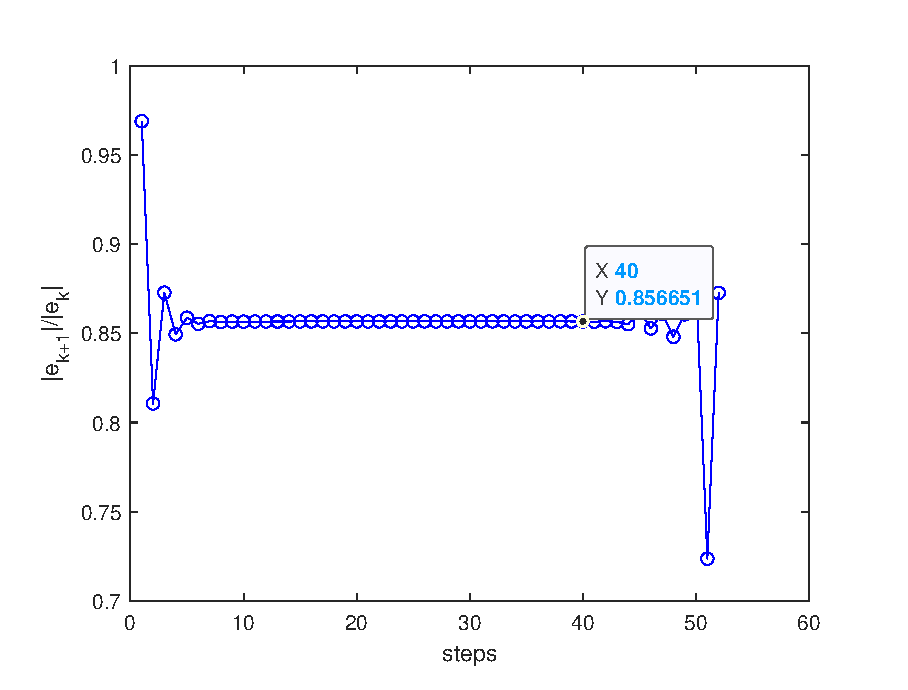
\includegraphics[width=14cm,height=10cm]{3_2_order.eps}
            \caption{练习6.5.2问题取$p=1$对数值收敛阶的观察} 
        \end{figure*}

        据图可见,使用割线法求解练习6.5.1问题的渐进收敛速度约为0.618,求解练习6.5.2问题的渐进收敛速度约为0.857,相较切线法收敛速度存在下降。
        \par
        \
        \par
        CPU执行时间见下表
        \begin{table}[htbp]%调节图片位置,h:浮动;t:顶部;b:底部;p:当前位置
            \centering
            \label{tab:1}  
            \begin{tabular}{ccc}%表格中的数据居中,c的个数为表格的列数
                \hline\hline\noalign{\smallskip}	
                \  & \texttt{Newton()} & \texttt{secant\_method()} \\
                \noalign{\smallskip}\hline\noalign{\smallskip}
                $f_1(x)$ & 0.000017 & 0.000018  \\
                $f_2(x)$ & 0.000022  & 0.000022 \\
                \noalign{\smallskip}\hline
            \end{tabular}
            \caption{切线法和割线法CPU运行时间比较(单位:秒)}
        \end{table}
        \par
        上述数据均是在程序执行100次后获得的运行时间,消除了Cache命中率对程序运行时间的影响。二者无明显差异,\texttt{Newton()}因迭代次数较少,CPU运行时间稍短,但本次实验的导数值计算均为$f'_1(x)$和$f'_2(x)$事先算好后封装的函数调用,减少了切线法的计算负担。
        
\section{小结}
    \par
    通过上述实验题,对非线性方程求解常用的Newton方法及其在有重根情形的修正算法进行了误差表现和收敛速度的数值观察,并与其近似求解手段割线法进行了收敛表现和CPU运行时间的比较。切线法经由合适的修正后具有较快的收敛速度和较高的收敛阶,但实际使用中导数值的计算具有困难,而割线法以收敛速度的一定程度下降为代价规避了导数值的计算,以一阶差商值代替导数值,在实际非线性方程求解问题中应根据$f(x)$的具体信息加以选择和修正处理。

    \begin{thebibliography}{99}  
        \bibitem{ref1}林成森. 数值计算方法(下册)[M]. 北京: 科学出版社, 2005.
    \end{thebibliography}
\end{document}
